% Complete Section 5.1, source PDF 61-64 / printed 51-54, including footnote 3 and both figures.
% block: primal-galerkin-heading page:61 type:section
\subsection{\BT{Galerkin discretization of the primal formulation}{原始表述的 Galerkin 离散化}}\label{sec:primal-galerkin}

% block: primal-galerkin-deficiencies pages:61,62 type:ordinary-paragraph
\BT{A simple approach to discretization of the Hodge Laplacian would be the application of Galerkin's method to the primal weak formulation \eqref{eq:hodge-primal-formulation}, i.e., restricting the trial and test functions to some finite dimensional subspace $V_h\subset V^k\cap V_k^*\cap\mathsf H^{k\perp}$. However, this approach suffers from two serious deficiencies, as we shall now show. First, we can anticipate some difficulty working with the condition $V_h\perp\mathsf H^k$, since in many problems, we do not know the space $\mathsf H^k$ explicitly and may not even know its dimension. We will return to this issue in a moment. Second, \emph{the primal approach may have difficulties even when there are no nonvanishing harmonic forms}. The difficulty here is that the space $V^k\cap V_k^*$ is not a standard Sobolev space, and it may be difficult to design a finite element subspace of it with good approximation properties. More precisely, the space may contain vector fields which are too singular to belong to $H^1$ or even to be approximated arbitrarily closely by $H^1$ vector fields. Such singular fields arise as solutions of the Hodge Laplacian on domains with nonconvex corners and in other situations, so this is a serious defect.}{离散化 Hodge Laplacian 的一种简单途径, 是将 Galerkin 方法应用于原始弱表述 \eqref{eq:hodge-primal-formulation}, 即把试探函数和检验函数限制在某个有限维子空间 $V_h\subset V^k\cap V_k^*\cap\mathsf H^{k\perp}$ 中. 但是, 这种途径存在两个严重缺陷, 下面予以说明. 首先, 可以预见, 条件 $V_h\perp\mathsf H^k$ 的处理会有困难, 因为在许多问题中, 我们并不明确知道空间 $\mathsf H^k$, 甚至可能不知道它的维数. 稍后将回到这个问题. 其次, \emph{即使不存在非零调和形式, 原始方法也可能遇到困难}. 这里的困难在于, 空间 $V^k\cap V_k^*$ 不是标准的 Sobolev 空间, 可能难以构造具有良好逼近性质的有限元子空间. 更准确地说, 该空间可能包含过于奇异的向量场, 它们既不属于 $H^1$, 甚至也无法被 $H^1$ 向量场任意精确地逼近. 在具有非凸角点的区域以及其他情形中, 这类奇异场会作为 Hodge Laplacian 的解出现, 因而这是一个严重的缺陷.}

% block: primal-galerkin-polygon page:62 type:ordinary-paragraph
\BT{As a simple example, suppose that $\Omega$ is a nonconvex simply connected polygon in the plane and consider the two-dimensional $L^2$ de Rham complex, for which the domain complex is}{作为一个简单例子, 设 $\Omega$ 是平面上的非凸单连通多边形, 考虑二维 $L^2$ de Rham 复形, 其定义域复形为}
\[
0\to H^1(\Omega)\xrightarrow{\operatorname{grad}}H(\operatorname{curl},\Omega)\xrightarrow{\operatorname{curl}}L^2(\Omega)\to0
\]
\BT{(here $\operatorname{curl}u=\partial u_2/\partial x_1-\partial u_1/\partial x_2$). Since the domain is simply connected there are no harmonic $1$-forms, and so the primal weak formulation \eqref{eq:hodge-r3-magnetic-primal} of the $k=1$ Hodge Laplacian for this complex seeks $u\in Y:=H(\operatorname{curl})\cap\mathring H(\operatorname{div})$ such that}{(这里 $\operatorname{curl}u=\partial u_2/\partial x_1-\partial u_1/\partial x_2$). 由于区域单连通, 不存在调和 $1$-形式, 因此此复形在 $k=1$ 时的 Hodge Laplacian 的原始弱表述 \eqref{eq:hodge-r3-magnetic-primal} 是求 $u\in Y:=H(\operatorname{curl})\cap\mathring H(\operatorname{div})$, 使得}
\begin{equation}\label{eq:primal-galerkin-polygon}
\int_\Omega[(\operatorname{curl}u)(\operatorname{curl}v)+(\operatorname{div}u)(\operatorname{div}v)]\,dx=\int_\Omega f\cdot v\,dx,\qquad v\in Y.
\end{equation}

% block: primal-galerkin-normal-space page:62 type:ordinary-paragraph
\begingroup\emergencystretch=1em
\BT{Let $H_n^1=H^1(\Omega;\mathbb R^2)\cap\mathring H(\operatorname{div})$ denote the space of $H^1$ vector fields with vanishing normal component on the boundary, which is a closed subspace of $H^1(\Omega;\mathbb R^2)$. Clearly $H_n^1\subset Y$. Moreover,}{用 $H_n^1=H^1(\Omega;\mathbb R^2)\cap\mathring H(\operatorname{div})$ 表示在边界上法向分量为零的 $H^1$ 向量场空间, 它是 $H^1(\Omega;\mathbb R^2)$ 的闭子空间. 显然 $H_n^1\subset Y$. 此外,}%
% block: polygon-vector-identity-footnote page:62 type:footnote
\footnote{\BT{This identity follows from a more general one:}{该恒等式可由下面更一般的恒等式导出:}
\[
\begin{aligned}
&\int\operatorname{curl}u\operatorname{curl}v\,dx+\int\operatorname{div}u\operatorname{div}v\,dx\\
&\quad=\int\operatorname{grad}u:\operatorname{grad}v\,dx+\sum_e\int_e\left(\frac{\partial u\cdot s}{\partial s}v\cdot n-\frac{\partial u\cdot n}{\partial s}v\cdot s\right)\,ds,\qquad u,v\in H^1(\Omega;\mathbb R^2);
\end{aligned}
\]
\BT{where the sum is over all the edges $e$ of the polygon $\Omega$ and $n$ and $s$ are the (constant) normal and tangent vectors on $e$. This is elementary for $u,v\in C^1(\bar\Omega;\mathbb R^2)$ (integration by parts). Each of the integrals appearing is a bilinear form of $u$ and $v$ bounded with respect to the $H^1$ norm, so we can extend by density. For example,}{其中对多边形 $\Omega$ 的所有边 $e$ 求和, $n$ 和 $s$ 是 $e$ 上的 (常) 法向量和切向量. 对 $u,v\in C^1(\bar\Omega;\mathbb R^2)$, 这是一个初等结论 (分部积分). 其中出现的每个积分都是 $u$ 和 $v$ 的双线性型, 且关于 $H^1$ 范数有界, 因此可利用稠密性延拓. 例如,}
\[
\begin{aligned}
\left|\int_e\frac{\partial u\cdot s}{\partial s}v\cdot n\right|&\leq\left\|\frac{\partial u\cdot s}{\partial s}\right\|_{H^{-1/2}(e)}\|v\cdot n\|_{H^{1/2}(e)}\\
&\leq\|u\cdot s\|_{H^{1/2}(e)}\|v\cdot n\|_{H^{1/2}(e)}\leq\|u\|_{H^1(\Omega)}\|v\|_{H^1(\Omega)}.
\end{aligned}
\]
}%
% block: polygon-vector-norm-identity page:62 type:equation
\[
\|\operatorname{curl}u\|^2+\|\operatorname{div}u\|^2=\|\operatorname{grad}u\|^2,\qquad u\in H_n^1.
\]
\par\endgroup

% block: primal-galerkin-closed-proper-subspace page:62 type:ordinary-paragraph
\BT{It follows that the restriction of the $Y$ norm (the norm of $H(\operatorname{div})\cap H(\operatorname{curl})$) to $H_n^1$ is equivalent to the full $H^1$ norm there. Since $H_n^1$ is closed in $H^1$, it is a \emph{closed} subspace of $Y$. Moreover, $H_n^1\ne Y$. This follows from the fact that a generic solution of the Neumann problem for Poisson's equation on a nonconvex polygon exhibits singular behavior near the reentrant corners, which precludes it belonging to $H^2$. Thus there exists $\phi\in H^1(\Omega)$ such that $\Delta\phi\in L^2(\Omega)$ and $\partial\phi/\partial n=0$ on $\partial\Omega$, but $\phi\notin H^2(\Omega)$. Setting $u=\operatorname{grad}\phi$ we see that $u\in Y$ but $u\notin H^1$.}{由此可知, $Y$ 范数 (即 $H(\operatorname{div})\cap H(\operatorname{curl})$ 的范数) 在 $H_n^1$ 上的限制, 与该空间上的完整 $H^1$ 范数等价. 由于 $H_n^1$ 在 $H^1$ 中闭, 它是 $Y$ 的\emph{闭}子空间. 此外, $H_n^1\ne Y$. 这是因为, 非凸多边形上的 Poisson 方程 Neumann 问题的一般解, 在凹角附近具有奇异行为, 从而不属于 $H^2$. 因此存在 $\phi\in H^1(\Omega)$, 满足 $\Delta\phi\in L^2(\Omega)$, 且在 $\partial\Omega$ 上有 $\partial\phi/\partial n=0$, 但 $\phi\notin H^2(\Omega)$. 令 $u=\operatorname{grad}\phi$, 可见 $u\in Y$, 但 $u\notin H^1$.}

% block: primal-galerkin-nonapproximation pages:62,63 type:ordinary-paragraph
\BT{In fact, this lack of $H^1$ regularity is typical of solutions of \eqref{eq:primal-galerkin-polygon}. For any such solution, we have $\inf_{v\in H_n^1}\|u-v\|_Y=\delta_u>0$, where $\delta_u$ is the distance of $u$ from the proper closed subspace $H_n^1$. This tells us that if the subspaces $V_h$ are contained in $H_n^1$, then the numerical solution $u_h\in V_h$ cannot converge to $u$. This is the case when $V_h$ is any subspace of $Y$ which consists of piecewise polynomials with respect to some triangulation. Indeed, the condition $V_h\subset H(\operatorname{curl})$ implies that the tangential components of any $v\in V_h$ must be continuous across triangle boundaries, and the fact that $V_h\subset H(\operatorname{div})$ implies that the normal components must be continuous. Thus $V_h$ consists of continuous piecewise polynomial functions, and so $V_h\subset H_n^1$.}{事实上, \eqref{eq:primal-galerkin-polygon} 的解通常就缺乏这种 $H^1$ 正则性. 对任一这样的解, 有 $\inf_{v\in H_n^1}\|u-v\|_Y=\delta_u>0$, 其中 $\delta_u$ 是 $u$ 到真闭子空间 $H_n^1$ 的距离. 这说明, 若子空间 $V_h$ 包含于 $H_n^1$, 则数值解 $u_h\in V_h$ 不可能收敛于 $u$. 当 $V_h$ 是 $Y$ 中由某一剖分上的分片多项式构成的任意子空间时, 情况就是如此. 事实上, 条件 $V_h\subset H(\operatorname{curl})$ 蕴含任意 $v\in V_h$ 的切向分量必须跨三角形边界连续, 而 $V_h\subset H(\operatorname{div})$ 蕴含法向分量必须连续. 因此 $V_h$ 由连续分片多项式函数构成, 从而 $V_h\subset H_n^1$.}

% block: primal-galerkin-l-shaped-figure page:63 type:figure
\begin{figure}[htbp]\centering
\includegraphics[page=63,trim=95bp 507bp 57bp 62bp,clip,width=.96\linewidth]{../input/source/Finite Element Exterior Calculus.pdf}
\caption{\BT{Finite element solution to the Hodge Laplacian problem on an L-shaped domain (with $f=(1,0)$). The left figure is calculated with a mixed method which is known to converge to the solution in $L^2$. The right figure is based on the primal formulation using $24{,}576$ piecewise linear elements. The primal-based numerical solution entirely misses the dominant behavior at the reentrant corner and produces a wholly inaccurate solution.}{L 形区域上的 Hodge Laplacian 问题的有限元解 (其中 $f=(1,0)$). 左图由混合方法计算, 已知该方法在 $L^2$ 中收敛于解. 右图基于原始表述, 使用 $24{,}576$ 个分片线性单元. 基于原始表述的数值解完全遗漏了凹角处的主导行为, 得到了完全不准确的解.}}\label{fig:primal-lagrange-failure}
\end{figure}

% block: primal-galerkin-nightmare page:63 type:ordinary-paragraph
\BT{In short, \emph{a standard finite element method based on the primal formulation does not generally converge to the solution $u$}. This behavior is illustrated in Figure~\ref{fig:primal-lagrange-failure}, which depicts a numerical analyst's nightmare. The figure on the right shows the numerical solution computed with what would seem to be a natural discretization: the finite element method based on the primal weak formulation, using continuous piecewise linear vector fields as trial functions. The method converges, as the mesh is refined, to what might be taken to be the solution but is, in fact, an altogether different vector field. In three dimensions, the situation is similar but worse, because then $H_n^1$ is a closed subspace of infinite codimension. See \BookCite{34} for an illuminating discussion.}{总之, \emph{基于原始表述的标准有限元方法一般并不收敛于解 $u$}. Figure~\ref{fig:primal-lagrange-failure} 展示了这种行为, 这正是数值分析工作者的噩梦. 右图给出了一种看似自然的离散方法算出的数值解: 基于原始弱表述的有限元方法, 以连续分片线性向量场为试探函数. 随着网格加密, 该方法收敛于一个可能被当作解的向量场, 但实际上它是一个完全不同的向量场. 三维情形类似, 而且更糟, 因为此时 $H_n^1$ 是无限余维的闭子空间. 文献 \BookCite{34} 给出了富有启发性的讨论.}

% block: primal-galerkin-earlier-eigenvalues page:63 type:ordinary-paragraph
\BT{We encountered this problem already in Chapter~\ref{chap:introduction} when we computed the eigenvalues of the vector Laplacian on a polygonal domain with a hole. Because of the reentrant corners, the true eigenfunctions are singular, and the standard finite element method cannot compute them accurately. This results in nonconvergence of the eigenvalues as well, as we saw in the example.}{在 Chapter~\ref{chap:introduction} 计算带孔多边形区域上向量 Laplacian 的特征值时, 我们已经遇到过这一问题. 由于存在凹角, 真正的特征函数是奇异的, 标准有限元方法无法准确计算它们. 正如该例中所见, 这也导致特征值不收敛.}

% block: primal-galerkin-harmonic-loss page:63 type:ordinary-paragraph
\BT{An independent difficulty with the primal formulation arises when there are harmonic forms. The difficulty is that we usually cannot arrange that the harmonic forms belong to the subspace $V_h$. The harmonic forms will generally be smooth functions, but not polynomials. Therefore, if the space $V_h$ is a finite element space, consisting of piecewise polynomials, it will not contain the any nonzero harmonic forms. The discrete problem, to find $u_h\in V_h$ such that}{当存在调和形式时, 原始表述还会遇到一个独立的困难. 困难在于, 通常无法使调和形式属于子空间 $V_h$. 调和形式一般是光滑函数, 但并非多项式. 因此, 如果空间 $V_h$ 是由分片多项式构成的有限元空间, 它将不包含任何非零调和形式. 于是离散问题, 即求 $u_h\in V_h$ 使得}
\[
\langle du_h,dv\rangle+\langle d^*u_h,d^*v\rangle=\langle f,v\rangle,\qquad v\in V_h,
\]
\BT{therefore has a unique solution (the bilinear form on the left-hand side defines an operator $V_h\to V_h'$ with zero kernel). Stated in other terms, the space of discrete harmonic forms vanishes. Therefore, the side condition $u\perp\mathsf H$ is lost on passage to the discrete level. The result, illustrated in Figure~\ref{fig:primal-harmonic-failure}, is that the discrete solution does not resemble the exact solution, even in order of magnitude. Another nightmare!}{具有唯一解 (左端的双线性型定义了一个核为零的算子 $V_h\to V_h'$). 换言之, 离散调和形式空间为零. 因此, 在转入离散层次时, 附加条件 $u\perp\mathsf H$ 丢失了. 结果如 Figure~\ref{fig:primal-harmonic-failure} 所示, 离散解与精确解甚至在数量级上都不相似. 又一场噩梦!}

% block: primal-galerkin-annulus-figure page:64 type:figure
\begin{figure}[htbp]\centering
\includegraphics[page=64,trim=96bp 513bp 63bp 62bp,clip,width=.96\linewidth]{../input/source/Finite Element Exterior Calculus.pdf}
\caption{\BT{Approximation of the Hodge Laplacian problem on an annulus ($f=(0,x)$). The true solution shown here on the left is an (accurate) approximation by a mixed method. The standard Galerkin solution using continuous piecewise linear vector fields, shown on the right, is totally different.}{环形区域上 Hodge Laplacian 问题的逼近 ($f=(0,x)$). 左图展示的真解是由混合方法得到的 (准确) 近似. 右图展示的使用连续分片线性向量场的标准 Galerkin 解则完全不同.}}\label{fig:primal-harmonic-failure}
\end{figure}
